\documentclass[10pt,a4paper]{article}
\usepackage[T1]{fontenc}
\usepackage[margin=22mm]{geometry}
\usepackage{amsmath,amssymb,booktabs,longtable,tabularx,graphicx,microtype}
\usepackage{placeins}
\usepackage[hidelinks]{hyperref}
\hypersetup{pdftitle={Supplementary methods and results: Handedness for Bangla writer identification: Oracle gains and predicted-attribute utility},pdfauthor={Tanzim Hasan Prappo; M. Shahidur Rahman}}
\usepackage[font=small,labelfont=bf]{caption}
% Generated from revised results.
\newcommand{\rWriters}{42}
\newcommand{\rLeft}{21}
\newcommand{\rImages}{336}
\newcommand{\rUnits}{5040}
\newcommand{\rInvalid}{39}
\newcommand{\rSettings}{120}
\newcommand{\rHandShared}{68.7}
\newcommand{\rHandOwn}{65.5}
\newcommand{\rHandWriter}{73.8}
\newcommand{\rLawN}{456}
\newcommand{\rLawR}{0.996}
\newcommand{\rLawMae}{1.5}
\newcommand{\rLawBias}{-0.9}
\newcommand{\rThresholdMed}{86}
\newcommand{\rThresholdMin}{55}
\newcommand{\rThresholdMax}{98}
\newcommand{\rKnownGain}{6.1}
\newcommand{\rKnownLo}{+5.1}
\newcommand{\rKnownHi}{+7.1}
\newcommand{\rFusionGain}{-0.6}
\newcommand{\rFusionLo}{-2.3}
\newcommand{\rFusionHi}{+0.9}
\newcommand{\rFilterGain}{-14.3}
\newcommand{\rFilterLo}{-19.3}
\newcommand{\rFilterHi}{-9.5}
\newcommand{\rLeakEn}{82.1}
\newcommand{\rLeakRandomMin}{52.4}
\newcommand{\rLeakRandomMax}{76.2}
\newcommand{\rBrierOwn}{0.204}
\newcommand{\rNllOwn}{0.602}
\newcommand{\rOracleVsRandom}{-0.8}
\newcommand{\rOracleVsRandomLo}{-1.8}
\newcommand{\rOracleVsRandomHi}{+0.2}
\newcommand{\rRandomKnownGain}{6.9}
\newcommand{\rBothGain}{+1.08}
\newcommand{\rBothLo}{+0.50}
\newcommand{\rBothHi}{+1.72}
\newcommand{\rExampleProduct}{31.4}
\newcommand{\rExampleFilter}{28.0}
\newcommand{\rExampleCondCorrect}{42.7}
\newcommand{\rExampleCondWrong}{58.0}

% Generated by code/make_fusion_robustness_paper.py
\newcommand{\rNestedGain}{-0.08}
\newcommand{\rNestedLo}{-1.13}
\newcommand{\rNestedHi}{+0.81}
\newcommand{\rNestedVsFixedGain}{+0.49}
\newcommand{\rNestedVsFixedLo}{-0.15}
\newcommand{\rNestedVsFixedHi}{+1.28}
\newcommand{\rNestedNllGain}{-0.010}
\newcommand{\rNestedNllLo}{-0.041}
\newcommand{\rNestedNllHi}{+0.024}
\newcommand{\rWeightMedian}{0.5}
\newcommand{\rWeightZero}{1.3}
\newcommand{\rTempLower}{0.8}
\newcommand{\rTempUpper}{2.6}
\newcommand{\rTempNearMedian}{1}
\newcommand{\rSeedAccuracyMin}{64.3}
\newcommand{\rSeedAccuracyMax}{66.7}
\newcommand{\rSeedDisagree}{2.4}
\newcommand{\rSeedGainMin}{-0.57}
\newcommand{\rSeedGainMax}{-0.50}
\newcommand{\rFixedOmitMin}{-0.76}
\newcommand{\rFixedOmitMax}{+0.01}
\newcommand{\rNestedOmitMin}{-0.24}
\newcommand{\rNestedOmitMax}{+0.22}
\newcommand{\rKnownOmitMin}{+5.91}
\newcommand{\rKnownOmitMax}{+6.26}
\newcommand{\rFilterOmitMin}{-14.77}
\newcommand{\rFilterOmitMax}{-13.10}
\newcommand{\rTempGainMin}{-1.81}
\newcommand{\rTempGainMax}{+0.04}

% Generated by code/run_margin_diagnostic.py
\newcommand{\rFixedRescued}{2.02}
\newcommand{\rFixedDamaged}{2.59}
\newcommand{\rNestedRescued}{1.33}
\newcommand{\rNestedDamaged}{1.42}

\renewcommand{\thesection}{S\arabic{section}}
\renewcommand{\thetable}{S\arabic{table}}
\renewcommand{\thefigure}{S\arabic{figure}}
\renewcommand{\theequation}{S\arabic{equation}}
\setlength{\parskip}{4pt}
\setlength{\parindent}{0pt}
\title{Supplementary methods and results\\[4pt]\large Handedness for Bangla writer identification: Oracle gains and predicted-attribute utility}
\author{Tanzim Hasan Prappo and M. Shahidur Rahman}
\date{}
\begin{document}
\maketitle
\vspace{-12pt}
This document accompanies the revised manuscript. The authoritative numerical outputs are in \path{results/wid_revision_2026-11-08/}; the original run is retained separately for provenance. Primary identification results in the revised article use selected-reference normalization and equal writer weights. The revisions and additional controls are retrospective.

\section{Data units, exclusion and weighting}
BanglaHand provides 336 photographs from 42 writers, 21 in each handedness group, with eight paragraphs per writer. Paragraphs 1--6 use shared prompts; 7--8 are self-chosen texts. The released metadata links every photograph to a pseudonymous writer and condition. No new participants or images were collected for this revision.

Each photograph supplies a full-paragraph unit ($n=1$) and $n=2,4,8$ horizontal strips, giving 5,040 candidate units. At 1,536-pixel image width, rows with ink fraction exceeding 0.01 define a text-row region through its 0.5th and 99.5th percentiles. For $n>1$, nominal equally spaced cuts are moved to a minimum in the smoothed row-ink profile. The smoothing standard deviation is 96/5 pixels; the search half-width is the smaller of 48 pixels and the text-block height divided by $3n$, with a minimum of three pixels. Row fractions transfer these boundaries to the other image scales. Whole-paragraph units use the complete image. Strips preserve the photograph's full width before representation-specific cropping.

A unit is invalid if the cropped high-resolution ink mask has fewer than 200 ink pixels, the 768-pixel mask has fewer than 50 ink pixels, contour/skeleton features cannot be computed, or their values are nonfinite. All representations share this validity mask. Exactly 39 strips are invalid; no paragraph is excluded. Table~\ref{tab:exclusions} gives their distribution. Images flagged for bottom-edge truncation in the dataset are retained; this analysis does not claim immunity to truncation.

\begin{table}[ht]
\centering\small
\caption{Candidate and excluded units by strip count, text condition and handedness. Excluded units are omitted from all representations.}\label{tab:exclusions}
\begin{tabular}{rrlrrr}\toprule
$n$ & Hand & Text & Candidate & Excluded & Retained\\\midrule
% Generated by code/make_revision_paper.py; do not edit.
1 & R & shared & 126 & 0 & 126 \\
1 & R & own & 42 & 0 & 42 \\
1 & L & shared & 126 & 0 & 126 \\
1 & L & own & 42 & 0 & 42 \\
2 & R & shared & 252 & 0 & 252 \\
2 & R & own & 84 & 0 & 84 \\
2 & L & shared & 252 & 0 & 252 \\
2 & L & own & 84 & 0 & 84 \\
4 & R & shared & 504 & 0 & 504 \\
4 & R & own & 168 & 0 & 168 \\
4 & L & shared & 504 & 0 & 504 \\
4 & L & own & 168 & 1 & 167 \\
8 & R & shared & 1008 & 6 & 1002 \\
8 & R & own & 336 & 16 & 320 \\
8 & L & shared & 1008 & 2 & 1006 \\
8 & L & own & 336 & 14 & 322 \\
\bottomrule

\end{tabular}
\end{table}

For a setting, the outcome is averaged across reference configurations for each valid query unit, then across units within its writer, then equally across the 42 writers. Each writer contributes equally even if strip exclusions leave different numbers of units. Across-setting summaries average the 120 setting-specific accuracies equally; they are not a pooled per-strip accuracy. Rows of the saved rank file contain the corresponding normalized analysis weight.

\section{Self-contained feature specifications}
All extraction is implemented in \texttt{code/wid\_features.py}, \texttt{hc183.py} and \texttt{stroke\_features.py}. Feature matrices are supplied so that the identification and control analyses can be reproduced without rerunning neural inference.

\textbf{HC-183.} A photograph is converted to grayscale and resized to width 768 with aspect ratio preserved using Lanczos interpolation. For grayscale intensity $I$ on the 0--255 scale, a Gaussian background estimate $B$ with standard deviation 17 pixels defines ink by $(B-I>17)\land(B>120)\land(I<205)$. A four-pixel border is cleared and a $2\times2$ binary opening is applied. Gradients of the mask smoothed with standard deviation 0.7 give nine-bin unsigned orientation histograms and ink density in each of $4\times4$ cells (160 values). Row and column ink projections each contribute seven quantiles (0, .1, .25, .5, .75, .9, 1), mean and standard deviation (18 values). Five area quantiles (.1, .25, .5, .75, .9) of connected components with at least three pixels complete the 183 features.

\textbf{STROKE.} The corresponding ink rule is evaluated at width 1,536, with background smoothing standard deviation 34, an eight-pixel cleared border and removal of connected objects smaller than 12 pixels. The text block is cropped using row and column ink fractions (thresholds 0.01 and 0.005), their 0.5th/99.5th percentiles and ten pixels of padding. Stroke width is twice the mean distance-transform value on the skeleton. A contour sampling length $L=\max(4,\operatorname{round}(2\,\mathrm{width}))$ controls feature scale. The 208 components comprise a 16-bin contour-direction histogram, a $12\times12$ hinge histogram, 12 turning-angle bins, 12 endpoint-direction bins, 12 skeleton-orientation bins, nine slant bins, and endpoint, junction and hole counts normalized by skeleton length. Static contours do not reveal pen movement order. The mask discards grayscale information, but this alone does not prove that every acquisition effect is removed.

\textbf{Frozen grayscale embeddings.} Grayscale images are resized to width 1,568 using Lanczos interpolation; the tile-selection mask is the nearest-neighbor resize of the 768-pixel HC-183 mask. Nonoverlapping $224\times224$ tiles with at least 1\% ink are retained; the bottom edge is padded with median grayscale intensity. If no tile meets the threshold, all tiles are used. Grayscale is repeated into three channels and normalized by ImageNet means $(.485,.456,.406)$ and standard deviations $(.229,.224,.225)$. The checkpoints are torchvision \texttt{ResNet18\_Weights.IMAGENET1K\_V1}, \texttt{EfficientNet\_B0\_Weights.IMAGENET1K\_V1} and \texttt{ViT\_B\_16\_Weights.IMAGENET1K\_V1}; final classification layers are removed. Mean tile embeddings have dimensions 512, 1,280 and 768. Models remain in evaluation mode without fine-tuning.

\textbf{Stroke-CNN.} The frozen ResNet-18 above instead receives black-on-white binary tiles from the cropped high-resolution mask. Bilinear resizing targets a stroke width of three pixels, with image dimensions at least 224 pixels; interpolation can produce antialiased edges. White padding completes the tile grid, and tiles require at least 2\% ink; if none qualify, all are retained. Input normalization and mean aggregation follow the grayscale embeddings. This representation has 512 components. Its name does not indicate a separately trained handwriting network.

\textbf{Adjusted HC-183.} Seven grayscale statistics (mean, standard deviation and .05/.25/.5/.75/.95 quantiles), together with mask ink density, form nuisance covariates. A linear regression with intercept removes their fitted contribution from HC-183. Regression coefficients are fitted within each outer or inner SVM training split, then applied to its training and held-out samples. The adjusted representation is a sensitivity check, not a guarantee of causal removal of acquisition confounding.

\section{Information available at every fitting stage}
The identification gallery is closed-set and includes the true query writer. This is separate from holding that writer out of \emph{attribute-model} training. Table~\ref{tab:nesting} distinguishes these information sources.

\paragraph{Evaluation versus deployment.} The 42 outer fits implement cross-validation, with the known writer identifier used to assign samples to a held-out fold. They do not constitute an inference algorithm that can select a model by an unknown query identity. A deployable unseen-writer pipeline would fit one attribute model and calibrator on development writers, select temperature and fusion weight using separate development predictions, freeze them, and apply the same fitted rule to every future query. Gallery templates and permitted gallery metadata would be formed at enrolment. This study estimates held-out-writer performance with the available cohort and does not validate such a frozen pipeline on a new cohort. Refitting with enrolled-writer pages changes the information regime and requires a separate enrolled-writer evaluation. The exploratory both-sided analysis in S6 uses that broader regime and is not a substitute for external validation.

\begin{table}[ht]
\caption{Fitting hierarchy for the revised primary analysis. The query writer remains enrolled for identity matching, but contributes no samples to its query-handedness model.}\label{tab:nesting}
\centering\small
\begin{tabularx}{\textwidth}{p{.22\textwidth}X}\toprule
Component & Permitted fitting data\\\midrule
Image descriptors & Fixed extraction rules and frozen ImageNet checkpoints; no writer-specific network training.\\
ID standardization & Only whole paragraphs selected as gallery references in the current configuration, from all enrolled writers. No queried paragraph or unused reference paragraph.\\
ID templates & Selected standardized, normalized references of the relevant gallery writer.\\
Outer attribute model for writer $w$ & Valid shared units of the same size from the other 41 writers. Neither shared nor self-chosen units of $w$.\\
Inner attribute preprocessing and SVM & Training writers in each of five stratified group folds inside the outer 41-writer set. Nuisance regression, if used, is refitted here.\\
Platt calibrator & Out-of-fold SVM scores and labels of the outer 41 training writers. The query writer is absent.\\
ID temperature for queries of $w$ & ID-score negative log loss on query writers other than $w$ in the same setting, equally weighted by writer. No attribute probabilities enter temperature fitting.\\
Primary fusion & Fixed unit weight on log attribute probability; no fitted handedness weight.\\\bottomrule
\end{tabularx}
\end{table}

The SVM uses scikit-learn \texttt{SVC(kernel="linear", C=0.1)} after training-set standardization. Inner calibration uses five shuffled stratified group folds (seed 2031). A logistic regression calibrator with $C=10^4$ is fitted to the out-of-fold raw scores. Thus calibration is estimated without the outer writer, but it is not guaranteed to be accurate for a new population. The 41-writer folds are nearly, rather than exactly, balanced by hand. For strips, retained unit counts can differ; the original attribute fitting uses unit-level training observations. Evaluation gives writers equal weight.

For a full-paragraph query, gallery templates use other whole paragraphs. For strips, the gallery still uses whole paragraphs. Cosine ties are resolved by fixed lexicographic gallery-writer order. The revised run found no exact ties at the maximum baseline score. The hard-filter implementation adds ten to matching-hand cosine scores, which is sufficient because cosine lies in $[-1,1]$; incompatible writers remain lower in the complete ranking rather than being physically deleted. For top-1, this is equivalent to exclusion in the present nonempty binary groups.

Temperature $T$ uses the grid $10^{\operatorname{linspace}(-3,0,31)}$. Minimizing mean ID negative log loss excludes the scored writer's query outcomes and uses equal mean loss per other writer. It may use references of the scored writer as impostor-gallery entries, as permitted by the declared closed-set protocol. The historical learned-weight outputs are omitted because their development attribute scores were not regenerated inside a second outer exclusion. The new nested comparison in Section~\ref{sec:supnested} corrects that limitation. Historical identification outputs are retained for traceability and do not supply revised identification results. Unchanged attribute-prediction controls are reused as explicitly noted in Section~S5.

\section{Filtering identity and known random partitions}
Let a random query be sampled according to the setting's writer-balanced weights. Define $C$ as correct query-handedness prediction and $K$ as correct top-1 with the true hand supplied. Because an incorrect binary decision puts the true writer below every member of a nonempty opposite-hand group,
\[
\{\text{filtered success}\}=C\cap K.
\]
Consequently, $A_{\mathrm{filter}}=aP(K\mid C)$ exactly, while $aA_{\mathrm{known}}$ requires zero covariance between the two correctness indicators. Cross-hand \emph{baseline identification} errors concern a different relationship and cannot establish this assumption.

The evaluated prediction models are HC-183, adjusted HC-183 and STROKE across all 120 settings, plus writer-level HC-183 on the 96 self-chosen-text settings. This gives $3\times120+96=456$ combinations. Writer-level HC-183 averages log-odds over both self-chosen paragraphs or their strips before predicting. It assumes those documents are already linked to the same questioned writer and uses more writing than a single query; it is a multi-document sensitivity analysis, not a deployable single-query result. The combination count is an analysis grid, not the number of independent experimental replications.

Known random-partition controls uniformly assign 21 writers to each of two groups, supplying the true query membership as well as gallery memberships. The same 2,000 partitions are applied across settings. For a query with $j$ baseline impostors outranking the true writer, every one must lie in the 21-member opposite group for filtered success. Its exact expected success under a uniform partition is
\begin{equation}
 P(\text{success}\mid j)=
 \begin{cases}
 \binom{21}{j}/\binom{41}{j},&0\leq j\leq21,\\
 0,&j>21.
 \end{cases}
\end{equation}
This also accounts for deterministic tie precedence if required. The exact expectation is compared with Monte Carlo partitions; the partition quantiles describe variation among partitions, not a confidence interval for a new population. A writer-bootstrap interval for handedness minus the exact partition expectation instead conditions on the fitted scores and observed gallery.

\begin{table}[ht]
\centering\small
\caption{Across-setting mean changes in top-1, percentage points. Intervals resample writers with common indices across settings, conditional on the observed gallery and fitted evidence.}\label{tab:aggregate}
\begin{tabular}{lrrr}\toprule
Contrast & Mean & 95\% interval & Sign-flip $p$\\\midrule
% Generated by code/make_revision_paper.py; do not edit.
Known hand vs none & +6.1 & [+5.1, +7.1] & 0.0001 \\
Predicted-query fusion vs none & -0.6 & [-2.3, +0.9] & 0.5402 \\
Predicted-query filter vs none & -14.3 & [-19.3, -9.5] & 0.0001 \\
Expected random partition vs none & +6.9 & [+6.4, +7.4] & 0.0001 \\
Known hand vs expected random partition & -0.8 & [-1.8, +0.2] & 0.1795 \\
\bottomrule

\end{tabular}
\end{table}

\begin{table}[ht]
\centering\small
\caption{Independence-product diagnostics, with conditional writer-bootstrap intervals. Bias and mean absolute error (MAE) are percentage points. Correlation pools the stated combinations; these are not independent replications.}
\begin{tabular}{lrrr}\toprule
Prediction model & Bias [95\% CI] & MAE [95\% CI] & Pearson $r$ [95\% CI]\\\midrule
% Generated by code/make_revision_paper.py; do not edit.
All combinations & -0.9 [-2.0, +0.1] & 1.5 [1.3, 2.5] & 0.996 [0.988, 0.997] \\
HC-183 & -0.6 [-1.8, +0.5] & 1.3 [1.0, 2.2] & 0.996 [0.989, 0.998] \\
HC-183 adjusted & -0.9 [-2.1, +0.3] & 1.4 [1.1, 2.4] & 0.995 [0.984, 0.997] \\
HC-183, linked texts & -0.6 [-2.1, +0.8] & 1.2 [1.1, 2.6] & 0.998 [0.989, 0.998] \\
STROKE & -1.7 [-3.1, -0.1] & 1.9 [1.4, 3.3] & 0.991 [0.974, 0.994] \\
\bottomrule

\end{tabular}
\end{table}

Cross-hand baseline errors concern the hand of the top-ranked incorrect writer, rather than the correctness-event independence in the filtering identity. Table~\ref{tab:crosshand} reports the ratio of writer-balanced cross-hand error to all error, averaged across settings before taking the ratio. Some representations show greater same-hand confusability than the uniform-impostor reference. Proximity to that reference does not establish independence.

\begin{table}[ht]
\centering\small
\caption{Share of baseline errors assigned to the opposite hand, with conditional 95\% writer-bootstrap intervals. A uniformly selected wrong writer would have opposite hand with probability $21/41=51.2\%$.}\label{tab:crosshand}
\begin{tabular}{lr}\toprule
Representation & Cross-hand error share [95\% CI], \%\\\midrule
% Generated by code/make_revision_paper.py; do not edit.
STROKE & 55.4 [43.6, 66.0] \\
HC-183 & 42.3 [36.5, 48.8] \\
ResNet-18 & 43.8 [38.9, 48.4] \\
EffNet-B0 & 47.4 [41.8, 53.4] \\
ViT-B/16 & 44.7 [38.4, 51.0] \\
Stroke-CNN & 52.4 [48.0, 57.1] \\
\bottomrule

\end{tabular}
\end{table}

\section{Calibration and writer-associated label controls}
Attribute calibration is evaluated from the outer held-writer-out predictions, separately by unit size and shared versus self-chosen text. Brier score is the writer-balanced mean of $(p-y)^2$; negative log loss is the mean of $\log(1+e^\ell)-y\ell$, evaluated stably. The uninformative balanced prediction has Brier score 0.25 and log loss $\log2$. Reliability plots use five fixed equal-width probability bins. Bin-level writer-bootstrap intervals account for writer clustering; sparse-bin uncertainty should not be interpreted as proof of good or poor calibration.

\begin{table}[ht]
\centering\small
\caption{Writer-held-out prediction and proper scoring rules on self-chosen paragraph queries. Intervals are conditional writer bootstraps.}\label{tab:calibration}
\begin{tabular}{lrrr}\toprule
Model & Accuracy [95\% CI], \% & Brier score & Negative log loss\\\midrule
% Generated by code/make_revision_paper.py; do not edit.
HC-183 & 65.5 [53.6, 77.4] & 0.204 & 0.602 \\
HC-183 adjusted & 61.9 [50.0, 73.8] & 0.244 & 0.684 \\
STROKE & 48.8 [35.7, 61.9] & 0.286 & 0.775 \\
\bottomrule

\end{tabular}
\end{table}

\begin{figure}[ht]
\centering
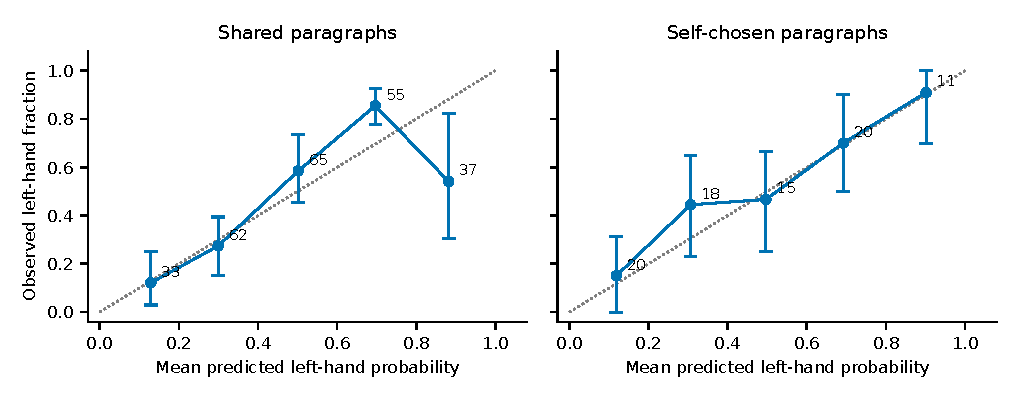
\includegraphics[width=\textwidth]{figures_revision/calibration.pdf}
\caption{Held-writer-out HC-183 calibration on paragraph queries. Five probability bins; vertical bars are conditional 95\% writer-bootstrap intervals. Bin counts and the underlying probabilities are supplied with the results.}
\end{figure}

The enrolment-trained label control fits the same predictor on all shared units and evaluates self-chosen texts. Shared-text outputs in the historical control use five-fold splits of paragraphs with writer overlap and an in-sample fit of the score calibrator; they are not used here to claim unbiased calibration. The clean comparison reported in the main text concerns self-chosen paragraphs excluded from training.

For 20 random 21/21 labelings, group 1 includes alternately 10 or 11 left-handed writers, and 11 or 10 right-handed writers. This makes random labels nearly unrelated to true hand while retaining equal group sizes. Figure~\ref{fig:labels} shows the random-label distribution as a diagnostic of writer-associated information. Fixed balanced labels can induce below-50\% leave-one-writer-out performance because the held-out label and training-set class composition are dependent. No nominal-chance test is used to interpret this structured null. Predictability of arbitrary labels establishes available writer-associated structure, not what fraction of true-handedness accuracy has that source.

\begin{figure}[ht]
\centering
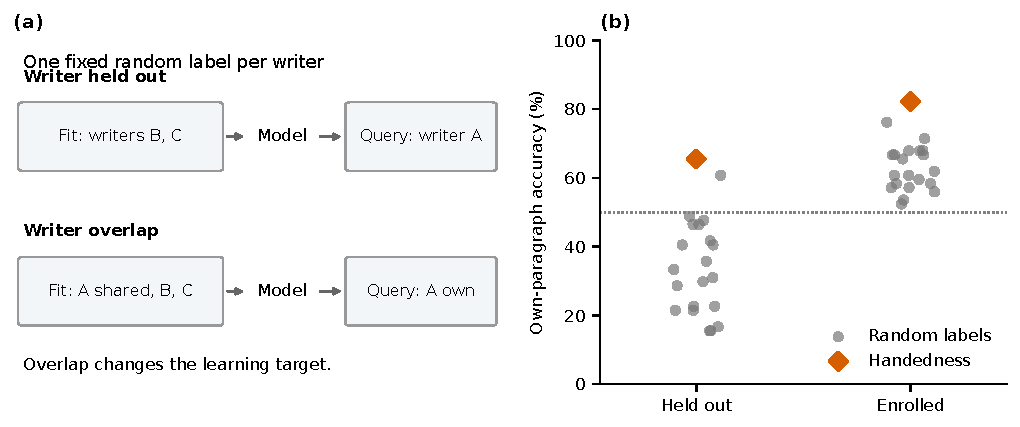
\includegraphics[width=\textwidth]{figures_revision/label_controls.pdf}
\caption{Writer-overlap diagnostic. (a) Schematic split designs: each writer has one fixed random label; training can exclude that writer or contain their shared paragraphs before testing their own text. (b) Own-paragraph prediction of genuine handedness and 20 random writer labelings. The 50\% line is descriptive, not a test against the structured held-out null. Gray points denote labelings. This control does not establish leakage in the primary writer-held-out experiment.}\label{fig:labels}
\end{figure}

\section{Both-predicted descriptor agreement}
\label{sec:both}
For exploratory both-sided prediction, we report only the 96 self-chosen-text settings. Shared-text queries would also enter the fitting data of impostor gallery-writer models, so their both-sided results are excluded from this reported comparison. Query log-odds are produced as above. A gallery writer's reference log-odds are averaged over its selected full paragraphs, using the attribute model that excluded that gallery writer. If $p_q$ and $p_w$ are the resulting probabilities, the agreement term is
\begin{equation}
 M(q,w)=\log\{p_qp_w+(1-p_q)(1-p_w)\},\qquad
 f_w=s_w/T+M(q,w).
\end{equation}
This is a descriptor-agreement score. It is not established as an identity posterior or evidence attributable specifically to physiological handedness. In particular, the model scoring an impostor gallery writer can have been trained on shared samples of the query writer. The procedure is therefore an enrolled-cohort, writer-cross-fitted diagnostic, not external prediction by a single attribute model trained without the entire queried cohort.

Controls use 20 random-label predictors with the same writer-level cross-fitting, those same scores centered and scaled per unit size to match the real score standard deviation, and 100 random HC-183 directions. Spread matching uses all valid cohort scores, including queried units; it is explicitly a transductive diagnostic matching procedure rather than deployable calibration. It neither matches every aspect of model complexity nor establishes a causal mechanism.

The revised both-predicted score changes top-1 by \rBothGain{} points on average (95\% conditional interval [\rBothLo, \rBothHi]). The controls use selected-reference ID normalization and save writer-level outcomes. Table~\ref{tab:both} reports both the empirical control-instance comparison and a direct paired writer comparison of the handedness score with the mean control. These are different uncertainty statements: the empirical exceedance fraction describes only the supplied control generation, while the bootstrap conditions on that ensemble and fitted gallery. The true handedness labeling is outside the support of the nearly hand-balanced random-label controls, so the exceedance fraction is not an exchangeable permutation-test $p$-value. Positive descriptor-consistency gains do not contradict the primary predicted-query result because the available gallery information and score rule differ.

\begin{table}[ht]
\centering\small
\caption{Exploratory both-sided fusion versus controls. All gains and differences are percentage points. Paired intervals compare handedness with the mean control; $e_{\rm ctrl}$ is the share of generated control instances at least as good as handedness, with the plus-one correction.}\label{tab:both}
\begin{tabular}{lrrrr}\toprule
Control & Instances & Control gain & Hand minus control [95\% CI] & $e_{\rm ctrl}$\\\midrule
% Generated by code/make_revision_paper.py; do not edit.
Random labels & 20 & +0.1 & +1.0 [+0.4, +1.6] & 0.048 \\
Random labels, scaled & 20 & +0.4 & +0.7 [+0.1, +1.3] & 0.048 \\
Random directions & 100 & +0.2 & +0.9 [+0.3, +1.5] & 0.010 \\
\bottomrule

\end{tabular}
\end{table}

\section{Synthetic evidence and prevalence sensitivity}
For a target attribute accuracy $a\in\{.50,.55,\ldots,1.00\}$ and $a<1$, Gaussian scores obey
\[
 z\mid h\sim N\big((2h-1)d/2,1\big),\quad
 d=2\Phi^{-1}(a),\quad\ell=dz.
\]
These are calibrated log-odds under the synthetic equal class prior. Noise is generated once for each distinct query unit in a draw and reused across all its reference configurations. The evidence is independent of fixed identification scores conditional on hand. At $a=.50$, fusion receives zero log-odds and filter ties are resolved by independent fair random decisions. At $a=1$, results are set to the exact oracle limit, avoiding finite substitutes for infinite separation. Two hundred draws are used per target accuracy and setting. ID temperature is estimated once from the same ID-only calibration procedure, not tuned to simulation outcomes.

Synthetic results demonstrate behavior under a chosen evidence family; they do not identify an accuracy threshold for arbitrary real predictors. Equal attribute accuracy does not fix confidence, calibration or the allocation of mistakes across identification margins. The complete simulation results are supplied and Fig.~\ref{fig:synthetic} shows the self-chosen paragraph, one-reference condition.

\begin{figure}[ht]
\centering
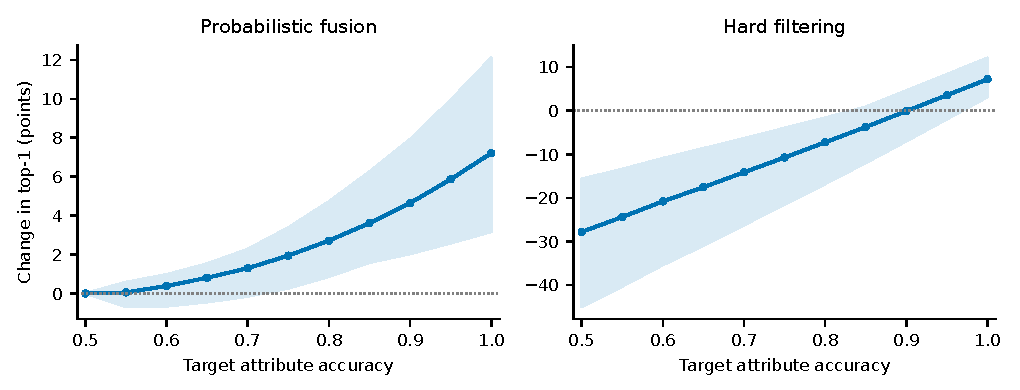
\includegraphics[width=\textwidth]{figures_revision/simulation.pdf}
\caption{Simulated independent calibrated evidence for self-chosen paragraphs with one reference. Curves average 200 draws; shaded ranges describe the spread over representations, not a sampling confidence interval. The exact oracle limit is used at 100\% accuracy.}\label{fig:synthetic}
\end{figure}

Prevalence experiments use 1,000 draws per condition, selecting 1, 2 or 3 of the 21 left-handed writers together with all 21 right-handed writers. Only queries from selected writers are retained, and normalization uses selected reference paragraphs of the selected gallery. ID-only temperatures fitted on the full 42-writer cohort, excluding each scored writer's query outcomes, remain fixed; they are not recalibrated in every reduced gallery. These perturbations reuse the cohort; they do not simulate recruitment from a new population. The original approximately balanced-source attribute log-odds remain unchanged for fusion and the ordinary filter. Only the prior-decision filter adds $\log(m/21)$ to query log-odds, where $m$ is the selected number of left-handed writers. This is a decision-rule sensitivity analysis, not a claim of exact posterior recalibration under label shift. Class-specific results are reported separately; a population-weighted utility would require a specified query prior and error-cost function. No casework recommendation or universal minority benefit is inferred from this sensitivity analysis.

\section{Properly nested fusion-weight selection}
\label{sec:supnested}
The fixed score rule assigns unit weight to log handedness evidence. To test a more flexible rule, we select a nonnegative weight by development negative log loss while retaining the same gallery, identity scores, outer query predictions and ID-only temperature. For outer writer $u$, the score is
\[
 f_{qj}=s_{qj}/T_u+\lambda_u\log p_q(h_j),\qquad
 \Lambda=\{0,.1,.2,.3,.5,.7,1,1.5,2,3,5\}.
\]
The development objective is
\[
 \lambda_u=\underset{\lambda\in\Lambda}{\arg\min}\;
 \frac1{41}\sum_{v\ne u}\overline{\mathrm{NLL}}_v
 \big(T_u,\lambda;\ell^{(-u,-F(v))}\big),
\]
where the bar denotes the same within-writer unit/configuration averaging used for primary accuracy, and $F(v)$ is the development writer fold containing $v$. Exact objective ties select the smaller weight. The grid and objective are fixed before this additional run, without choosing a rule from its test results. This is a post-review exploratory comparison, not preregistration.

For each outer exclusion, the remaining 41 writers are split into five stratified writer folds (seed 2031). The HC-183 SVM generating each development fold's probabilities trains on only the remaining 32 or 33 writers. Its standardization and an additional five-fold writer-group Platt calibration are fitted entirely inside that training subset. Thus the outer writer and every development validation writer are absent from all relevant attribute fits. The final attribute predictor used on outer query $u$ is the existing model trained and calibrated on the other 41 writers. Development models therefore have fewer training writers than that final outer predictor, a normal finite-sample cross-validation distinction.

The temperature is the same ID-only $T_u$ as for fixed fusion; it is not retuned against outer-writer outcomes or attribute probabilities. All 42 gallery templates and known gallery hands remain available as candidate metadata, including writer $u$ as an impostor for development queries. This matches the declared closed-gallery information set. It does not expose the questioned samples or query targets of $u$ to development fitting. The evaluation estimates a writer-held-out calibration procedure conditional on this gallery; it is not a prospective validation of one universal fitted temperature/weight on unseen casework.

The values $\lambda=0$ and $\lambda=1$ recover baseline ranking and fixed fusion respectively. Automated checks verify these comparator outcomes against the separately generated primary results. Development loss is no larger than either comparator's loss by construction; held-out performance need not improve. The objective is log loss rather than top-1 accuracy. An equivalent two-hand log-sum-exp calculation is checked against the full 42-candidate loss, and changing outer-query targets or their development-score placeholders does not change selected weights. Fold manifests document 840 development models and their inner calibration exclusions.

\begin{table}[ht]
\centering\small
\caption{Nested learned-weight contrasts over all 120 settings. Positive top-1 differences favor the learned rule; negative NLL differences favor it. All intervals are conditional 95\% writer bootstraps, with common resampled writer indices across settings.}
\begin{tabular}{llrr}\toprule
Metric & Contrast & Mean [95\% CI] & Sign-flip $p$\\\midrule
% Generated by code/make_revision_paper.py; do not edit.
Top-1 (points) & Nested minus none & -0.08 [-1.13, +0.81] & 0.8784 \\
Top-1 (points) & Nested minus fixed & +0.49 [-0.15, +1.28] & 0.2205 \\
NLL (nats) & Nested minus none & -0.010 [-0.041, +0.024] & 0.5418 \\
NLL (nats) & Nested minus fixed & -0.022 [-0.054, +0.006] & 0.1784 \\
\bottomrule

\end{tabular}
\end{table}

The learned-rule comparisons against no fusion and fixed fusion in the four designated settings form one eight-comparison Holm family. These tests, and their uncertainty, are reported in the main article. The paired bootstrap resamples fitted writer outcomes rather than refitting the complete nested procedure; it therefore does not quantify all uncertainty from data-dependent parameter selection. Full writer-level outcomes and validation losses are supplied for all settings.

\begin{table}[ht]
\centering\small
\caption{Selected weight distributions across 42 outer writers and 20 settings per representation. Frequencies describe correlated writer/setting fits, not independent experimental repetitions. IQR: interquartile range.}
\begin{tabular}{lrrrr}\toprule
Representation & Median [IQR] & $\lambda=0$, \% & $\lambda=1$, \% & Range\\\midrule
% Generated by code/make_revision_paper.py; do not edit.
STROKE & 0.7 [0.3, 1.0] & 1.5 & 24.3 & 0.0--5.0 \\
HC-183 & 0.3 [0.2, 0.5] & 2.6 & 1.9 & 0.0--1.0 \\
ResNet-18 & 0.5 [0.3, 0.7] & 2.9 & 13.2 & 0.0--1.5 \\
EffNet-B0 & 0.5 [0.5, 0.7] & 0.4 & 20.2 & 0.0--1.5 \\
ViT-B/16 & 0.5 [0.5, 0.7] & 0.2 & 16.7 & 0.0--1.5 \\
Stroke-CNN & 0.5 [0.5, 1.0] & 0.0 & 22.5 & 0.1--1.5 \\
\bottomrule

\end{tabular}
\end{table}

\section{Uncertainty and within-cohort robustness diagnostics}
\label{sec:suprobust}
Figure~\ref{fig:robustness} summarizes the within-cohort parameter and prediction diagnostics.
\subsection{Temperature selection and loss sensitivity}
For every setting and held-out writer, we retain the writer-balanced development ID loss at all 31 candidate temperatures, the selected value, the gap to the second-best value, and the number of temperatures within 0.01 nats of the minimum. This tolerance is a descriptive measure of a loss plateau, not a confidence level or a threshold for practical importance. Table~\ref{tab:tempdiag} reports boundary frequencies and observed ranges. Boundary selection alone does not establish that the optimum is misspecified, particularly when several small temperatures give nearly identical loss.

\begin{table}[ht]
\centering\small
\caption{ID-only temperature diagnostics. Lower/upper: percentage of fits selecting $10^{-3}$ or 1. Near-optimal: median number of grid candidates within 0.01 development NLL nats of the selected minimum.}\label{tab:tempdiag}
\begin{tabular}{lrrrrr}\toprule
Representation & Median $T$ & Range & Lower, \% & Upper, \% & Near-optimal\\\midrule
% Generated by code/make_revision_paper.py; do not edit.
STROKE & 0.0501 & 0.0010--0.0794 & 5.0 & 0.0 & 1 \\
HC-183 & 0.0794 & 0.0398--0.1259 & 0.0 & 0.0 & 1 \\
ResNet-18 & 0.0794 & 0.0398--0.1585 & 0.0 & 0.0 & 1 \\
EffNet-B0 & 0.0794 & 0.0398--0.1995 & 0.0 & 0.0 & 1 \\
ViT-B/16 & 0.0794 & 0.0398--0.1995 & 0.0 & 0.0 & 1 \\
Stroke-CNN & 0.1885 & 0.0398--1.0000 & 0.0 & 15.8 & 2 \\
\bottomrule

\end{tabular}
\end{table}

We also evaluate fixed, outcome-independent multipliers $c=.5,1,2$ of each selected temperature, without clipping them to the original grid. For ranking, $s/(cT)+M$ is equivalent to $s/T+cM$. This perturbation therefore probes the relative attribute weight, rather than providing an independent source of evidence beyond the learned-weight comparison. Table~\ref{tab:tempsensitivity} gives paired writer uncertainty and the associated fused log loss. No multiplier is selected as a replacement primary rule after inspecting these outcomes.

\begin{table}[ht]
\centering\small
\caption{Fixed temperature-multiplier sensitivity over all 120 settings. Top-1 changes are relative to no fusion, in percentage points; NLL is the absolute fused log loss in nats. Intervals condition on the fitted gallery and predictions.}\label{tab:tempsensitivity}
\begin{tabular}{rrr}\toprule
Multiplier $c$ & Top-1 change [95\% CI] & Fused NLL [95\% CI]\\\midrule
% Generated by code/make_revision_paper.py; do not edit.
0.5 & +0.04 [-0.98, +0.90] & 2.226 [1.950, 2.536] \\
1 & -0.57 [-2.37, +0.91] & 1.879 [1.710, 2.062] \\
2 & -1.81 [-4.45, +0.35] & 2.108 [1.981, 2.242] \\
\bottomrule

\end{tabular}
\end{table}

\subsection{Prediction variability from calibration partitions}
The primary attribute pipeline uses grouped calibration seed 2031. We repeat it with seeds 2032, 2033 and 2034, changing only the inner calibration partitions. Every full outer SVM is refitted on the same training writers, and its raw decision scores are verified unchanged within numerical tolerance. The resulting probability differences therefore characterize calibration-partition variability, not neural initialization, a new feature extractor, independent participants or new datasets.

Table~\ref{tab:seeddiag} reports the self-chosen-paragraph attribute metrics and identification changes for every seed, retaining 2031 as the primary analysis. We save each unit's probability mean, standard deviation, range, and whether its predicted hand changes at least once across the four partitions. These are correlated partition replicates; they are not averaged as four independent studies, and the best seed is not selected. Each seed-specific interval resamples writers conditional on that seed's fitted predictions.

\begin{table}[ht]
\centering\small
\caption{Calibration-partition sensitivity. Attribute metrics use self-chosen paragraphs; fusion changes average all 120 settings and are in percentage points. Accuracy intervals and fusion intervals are conditional writer bootstraps.}\label{tab:seeddiag}
\begin{tabular}{rrrrr}\toprule
Seed & Hand accuracy [95\% CI], \% & Brier & NLL & Fixed fusion change [95\% CI]\\\midrule
% Generated by code/make_revision_paper.py; do not edit.
2031 & 65.5 [53.6, 77.4] & 0.204 & 0.602 & -0.57 [-2.37, +0.91] \\
2032 & 66.7 [54.8, 78.6] & 0.201 & 0.594 & -0.50 [-2.13, +0.83] \\
2033 & 64.3 [52.4, 76.2] & 0.202 & 0.599 & -0.56 [-2.33, +0.90] \\
2034 & 65.5 [53.6, 77.4] & 0.205 & 0.606 & -0.52 [-2.20, +0.86] \\
\bottomrule

\end{tabular}
\end{table}

\subsection{Evaluation-writer influence and class-specific effects}
For each writer, we omit that writer only from evaluation averaging, keeping the 42-writer gallery, fitted models, selected parameters and query predictions fixed. The remaining writers are reweighted to give each hand one half of the total weight. These are influence diagnostics, not reduced-gallery identification experiments, full leave-one-writer-out model refits or independent validation. All 42 writers remain in the primary results; neither prediction errors nor influence values constitute an exclusion criterion.

Table~\ref{tab:writerinfluence} gives the range across all 42 omissions and identifies the largest change. Omission ranges are descriptive ranges, not 95\% confidence intervals. In particular, a near-zero fusion mean can change sign under an omission without demonstrating either a benefit or a harmful effect. The full writer list, four designated-setting sensitivities and class-specific estimates are included in the numerical outputs. Table~\ref{tab:classeffects} reports the latter averaged across settings.

\begin{table}[ht]
\centering\small
\caption{Fixed-gallery evaluation-writer influence on mean top-1 gain, in percentage points. Each hand retains total weight 0.5 after omission; no models are refitted.}\label{tab:writerinfluence}
\begin{tabular}{lrrrr}\toprule
Method & All writers & Omission range & Largest change & Writer\\\midrule
% Generated by code/make_revision_paper.py; do not edit.
Known & +6.11 & [+5.91, +6.26] & 0.19 & L\_p5 \\
Fixed fusion & -0.57 & [-0.76, +0.01] & 0.58 & R\_p21 \\
Nested fusion & -0.08 & [-0.24, +0.22] & 0.30 & R\_p21 \\
Hard filter & -14.29 & [-14.77, -13.10] & 1.19 & R\_p21 \\
\bottomrule

\end{tabular}
\end{table}

\begin{table}[ht]
\centering\small
\caption{Class-specific top-1 changes from no fusion, percentage points, averaged over all settings with conditional writer-bootstrap intervals. These are observed-cohort subgroup summaries.}\label{tab:classeffects}
\begin{tabular}{lrr}\toprule
Method & Left-handed [95\% CI] & Right-handed [95\% CI]\\\midrule
% Generated by code/make_revision_paper.py; do not edit.
Known & +7.17 [+5.56, +8.91] & +5.05 [+4.00, +6.14] \\
Fixed fusion & -0.08 [-2.32, +1.67] & -1.05 [-4.04, +1.08] \\
Nested fusion & +0.14 [-1.21, +1.24] & -0.31 [-1.97, +0.97] \\
Hard filter & -14.21 [-21.31, -7.70] & -14.37 [-21.82, -7.83] \\
\bottomrule

\end{tabular}
\end{table}

\begin{figure}[!ht]
\centering
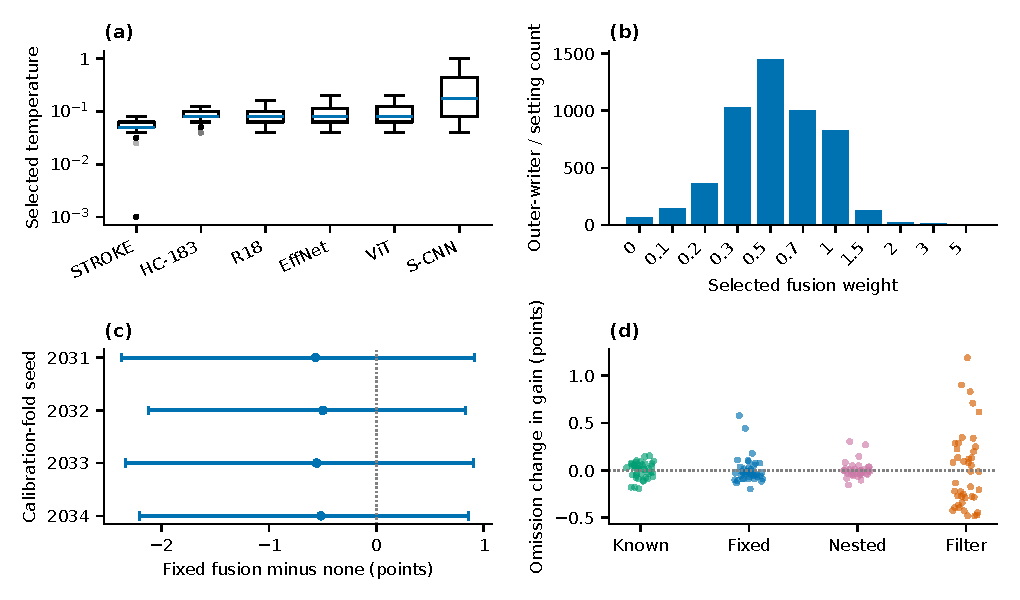
\includegraphics[width=\textwidth]{figures_revision/fusion_robustness.pdf}
\caption{Within-cohort diagnostics. (a) Selected temperature distributions across outer-writer/setting fits; boxes show quartiles, whiskers extend to 1.5 IQR and points show values outside them. (b) Learned-weight frequencies across the 5,040 fits. (c) Fixed-fusion mean differences and conditional writer-bootstrap intervals for each calibration partition. (d) Changes in mean gain after each evaluation-writer omission. None of these panels represents independent-dataset validation.}\label{fig:robustness}
\end{figure}

\FloatBarrier
\section{Decision margins and opposing fusion effects}
\label{sec:margins}
This retrospective diagnostic reuses the original calibrated HC-183 query log-odds and the already selected temperatures and nested weights. No parameter is refitted and all 42 writers and 120 settings remain. Let $w^*$ be the true writer, $K_q$ the event that it leads all same-hand candidates, and define
\[
 m_q=\frac{s_{qw^*}-\max_{j:h_j\ne h_{w^*}}s_{qj}}{T_q},\qquad
 r_q=\log\frac{p_q(h_{w^*})}{p_q(1-h_{w^*})}.
\]
Since the attribute term is constant within each hand group, fused top-1 success, away from ties, is exactly $K_q\cap\{m_q+\lambda_qr_q>0\}$. The computation also implements the fixed candidate-order rule for ties. This is an algebraic decomposition of the tested rule, not an additional prediction model. The true hand and identity are used for retrospective analysis only. It follows that fusion cannot repair a wrong within-hand ordering; it can only change the competition between the two groups.

A rescued decision is incorrect before fusion and correct afterwards; a damaged decision is correct before fusion and incorrect afterwards. Their difference equals the net top-1 change for every query/reference decision. The same equal-unit, equal-writer and equal-setting averaging as the main analysis gives fixed-fusion rescue and damage rates of \rFixedRescued\% and \rFixedDamaged\%, respectively; nested weighting gives \rNestedRescued\% and \rNestedDamaged\%. Thus a small mean change combines opposing changes rather than indicating that the attribute never affects ranking. The plot illustrates how signed attribute evidence interacts with the identity margin.

Intervals use 10,000 hand-stratified writer bootstraps (seed 20361109), with the same writer indices for all contrasts and settings. They are descriptive marginal intervals conditional on the gallery, predictions and selected parameters. The individual illustrated decisions share queries and writers and are not independent observations. Machine-readable writer outcomes, intervals, the illustrative decisions and input hashes are supplied as \path{margin_writer_outcomes.csv}, \path{margin_effect_intervals.csv}, \path{margin_example.csv} and \path{margin_validation.json}. Every reconstructed decision is compared with direct candidate-score ranking; writer-level fused accuracies are independently matched to the existing fixed and nested outputs.

\begin{figure}[ht]
\centering
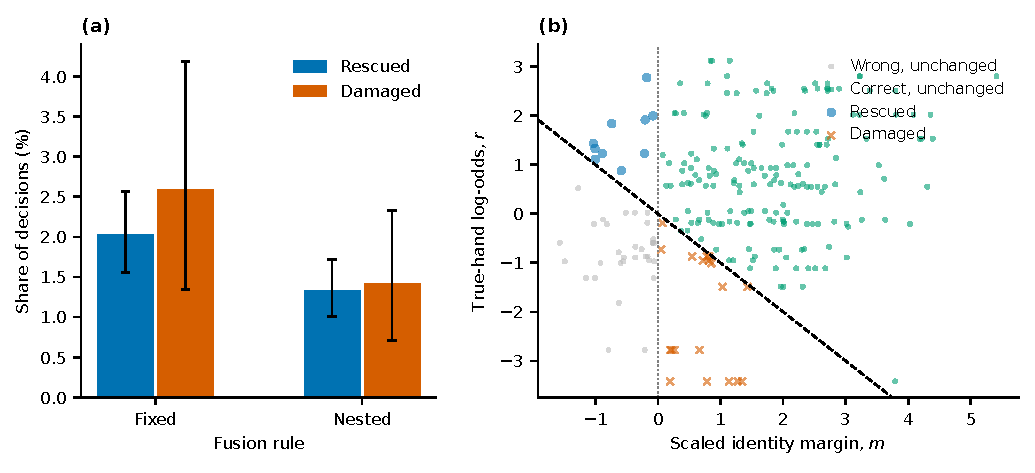
\includegraphics[width=\textwidth]{figures_revision/margin_diagnostic.pdf}
\caption{Decision changes and margin diagnostic. (a) Rescued and damaged decisions under fixed and nested fusion, averaging all 120 settings with equal writer weights; bars are marginal conditional 95\% writer-bootstrap intervals. (b) HC-183, self-chosen full paragraphs and one reference, fixed fusion: only decisions for which the true writer leads its hand group are plotted. The vertical line is the baseline boundary $m=0$; the dashed line is the fusion boundary $m+r=0$. Points above the dashed line succeed after fusion. Each point is a query/reference choice; repeated choices are correlated. The true-hand axes are retrospective diagnostics, not available prediction inputs.}
\label{fig:margins}
\end{figure}

\FloatBarrier
\section{Complete revised identification grid}
Table~\ref{tab:grid} reports all 120 settings for the primary HC-183 query predictor, including fixed and nested learned-weight fusion. The machine-readable results additionally contain top-5 accuracy, reciprocal rank, alternative handedness models, writer-level outcomes, temperatures and paired intervals. ``Shared'' uses the other five prompt pages as references. ``Own'' uses self-chosen query texts. Query size $n=1$ is a whole paragraph; larger $n$ is the number of strips per page. Thresholds are $A_{\rm none}/A_{\rm known}$ under the independence approximation, not empirically established universal requirements.

\small
\begin{longtable}{llrrrrrrrr}
\caption{Complete revised identification results, accuracy and approximate threshold in \%.}\label{tab:grid}\\
\toprule
Representation & Text & $n$ & $k$ & None & Known & Fixed & Nested & Filter & Threshold\\\midrule
\endfirsthead
\multicolumn{10}{l}{Table~\thetable{} continued}\\\toprule
Representation & Text & $n$ & $k$ & None & Known & Fixed & Nested & Filter & Threshold\\\midrule
\endhead
\bottomrule\endfoot
% Generated by code/make_revision_paper.py; do not edit.
STROKE & shared & 1 & 5 & 100.0 & 100.0 & 100.0 & 100.0 & 68.7 & 100.0 \\
STROKE & shared & 2 & 5 & 99.2 & 99.4 & 99.2 & 99.2 & 65.3 & 99.8 \\
STROKE & shared & 4 & 5 & 96.1 & 96.9 & 95.7 & 95.7 & 63.7 & 99.2 \\
STROKE & shared & 8 & 5 & 86.6 & 88.7 & 86.7 & 86.7 & 56.5 & 97.6 \\
STROKE & own & 1 & 1 & 92.3 & 95.4 & 93.3 & 92.5 & 62.3 & 96.7 \\
STROKE & own & 2 & 1 & 87.7 & 91.0 & 87.0 & 87.7 & 59.3 & 96.4 \\
STROKE & own & 4 & 1 & 82.8 & 86.9 & 83.4 & 83.6 & 57.0 & 95.3 \\
STROKE & own & 8 & 1 & 68.4 & 72.8 & 67.9 & 68.5 & 45.1 & 94.0 \\
STROKE & own & 1 & 2 & 94.9 & 97.3 & 95.5 & 94.9 & 63.7 & 97.6 \\
STROKE & own & 2 & 2 & 91.6 & 93.6 & 90.8 & 91.3 & 61.2 & 97.9 \\
STROKE & own & 4 & 2 & 86.5 & 90.0 & 86.8 & 87.1 & 59.3 & 96.2 \\
STROKE & own & 8 & 2 & 71.4 & 75.3 & 70.9 & 71.8 & 46.9 & 94.8 \\
STROKE & own & 1 & 3 & 95.2 & 97.4 & 95.5 & 95.2 & 63.9 & 97.7 \\
STROKE & own & 2 & 3 & 92.6 & 94.4 & 92.0 & 92.3 & 62.1 & 98.1 \\
STROKE & own & 4 & 3 & 87.9 & 91.0 & 88.3 & 88.5 & 60.2 & 96.6 \\
STROKE & own & 8 & 3 & 72.4 & 76.1 & 71.8 & 72.6 & 47.4 & 95.2 \\
STROKE & own & 1 & 6 & 95.2 & 98.8 & 96.4 & 95.2 & 65.5 & 96.4 \\
STROKE & own & 2 & 6 & 92.9 & 94.6 & 91.7 & 92.3 & 61.9 & 98.1 \\
STROKE & own & 4 & 6 & 89.0 & 91.1 & 88.7 & 89.0 & 60.0 & 97.7 \\
STROKE & own & 8 & 6 & 72.6 & 76.2 & 72.2 & 73.3 & 47.8 & 95.4 \\
HC-183 & shared & 1 & 5 & 82.9 & 86.1 & 80.6 & 82.9 & 57.9 & 96.3 \\
HC-183 & shared & 2 & 5 & 67.1 & 74.0 & 65.1 & 67.3 & 48.6 & 90.6 \\
HC-183 & shared & 4 & 5 & 42.3 & 51.4 & 41.3 & 41.8 & 34.0 & 82.2 \\
HC-183 & shared & 8 & 5 & 25.4 & 35.2 & 24.6 & 24.7 & 21.9 & 72.2 \\
HC-183 & own & 1 & 1 & 39.7 & 48.0 & 37.9 & 38.5 & 28.0 & 82.6 \\
HC-183 & own & 2 & 1 & 35.2 & 43.3 & 34.1 & 34.1 & 29.0 & 81.4 \\
HC-183 & own & 4 & 1 & 23.3 & 31.3 & 22.6 & 23.0 & 19.0 & 74.6 \\
HC-183 & own & 8 & 1 & 14.2 & 21.7 & 14.1 & 14.1 & 11.8 & 65.6 \\
HC-183 & own & 1 & 2 & 47.4 & 53.4 & 43.1 & 45.3 & 30.8 & 88.7 \\
HC-183 & own & 2 & 2 & 43.4 & 51.2 & 41.2 & 42.5 & 34.5 & 84.7 \\
HC-183 & own & 4 & 2 & 27.3 & 35.3 & 26.5 & 27.1 & 22.4 & 77.4 \\
HC-183 & own & 8 & 2 & 17.0 & 25.8 & 16.5 & 16.9 & 14.3 & 65.9 \\
HC-183 & own & 1 & 3 & 51.4 & 57.4 & 48.0 & 50.5 & 33.7 & 89.4 \\
HC-183 & own & 2 & 3 & 47.0 & 54.5 & 44.8 & 46.7 & 37.1 & 86.3 \\
HC-183 & own & 4 & 3 & 29.7 & 38.4 & 29.1 & 29.7 & 24.0 & 77.5 \\
HC-183 & own & 8 & 3 & 18.7 & 28.1 & 17.6 & 18.6 & 15.5 & 66.6 \\
HC-183 & own & 1 & 6 & 57.1 & 61.9 & 54.8 & 54.8 & 36.9 & 92.3 \\
HC-183 & own & 2 & 6 & 54.8 & 60.1 & 50.6 & 53.6 & 40.5 & 91.1 \\
HC-183 & own & 4 & 6 & 33.0 & 42.9 & 32.1 & 32.7 & 25.6 & 77.1 \\
HC-183 & own & 8 & 6 & 21.3 & 30.8 & 19.3 & 20.7 & 16.8 & 69.0 \\
ResNet-18 & shared & 1 & 5 & 96.8 & 96.8 & 96.0 & 96.4 & 66.7 & 100.0 \\
ResNet-18 & shared & 2 & 5 & 80.4 & 85.3 & 79.0 & 79.4 & 55.6 & 94.2 \\
ResNet-18 & shared & 4 & 5 & 63.8 & 70.2 & 62.9 & 63.5 & 46.1 & 90.8 \\
ResNet-18 & shared & 8 & 5 & 17.4 & 24.8 & 18.0 & 17.8 & 17.0 & 70.4 \\
ResNet-18 & own & 1 & 1 & 62.9 & 67.9 & 62.1 & 62.7 & 42.3 & 92.7 \\
ResNet-18 & own & 2 & 1 & 43.8 & 50.8 & 44.5 & 44.4 & 34.7 & 86.3 \\
ResNet-18 & own & 4 & 1 & 35.0 & 42.6 & 34.6 & 35.0 & 29.6 & 82.2 \\
ResNet-18 & own & 8 & 1 & 10.4 & 18.0 & 11.1 & 10.8 & 11.9 & 57.5 \\
ResNet-18 & own & 1 & 2 & 73.1 & 77.3 & 72.5 & 72.7 & 48.8 & 94.6 \\
ResNet-18 & own & 2 & 2 & 52.6 & 58.8 & 51.7 & 52.5 & 40.0 & 89.4 \\
ResNet-18 & own & 4 & 2 & 40.4 & 46.8 & 39.7 & 40.2 & 32.2 & 86.4 \\
ResNet-18 & own & 8 & 2 & 11.2 & 17.4 & 11.7 & 11.3 & 12.1 & 64.0 \\
ResNet-18 & own & 1 & 3 & 77.7 & 82.1 & 77.2 & 77.9 & 52.6 & 94.7 \\
ResNet-18 & own & 2 & 3 & 55.9 & 61.6 & 55.1 & 55.8 & 42.2 & 90.8 \\
ResNet-18 & own & 4 & 3 & 43.1 & 48.7 & 42.2 & 42.8 & 33.7 & 88.4 \\
ResNet-18 & own & 8 & 3 & 11.7 & 17.9 & 12.2 & 11.7 & 12.5 & 65.2 \\
ResNet-18 & own & 1 & 6 & 83.3 & 85.7 & 81.0 & 83.3 & 54.8 & 97.2 \\
ResNet-18 & own & 2 & 6 & 60.1 & 65.5 & 58.9 & 58.9 & 45.2 & 91.8 \\
ResNet-18 & own & 4 & 6 & 47.4 & 51.7 & 46.0 & 46.6 & 35.8 & 91.9 \\
ResNet-18 & own & 8 & 6 & 12.3 & 18.8 & 12.7 & 12.0 & 13.1 & 65.4 \\
EffNet-B0 & shared & 1 & 5 & 96.0 & 96.8 & 96.0 & 96.0 & 65.9 & 99.2 \\
EffNet-B0 & shared & 2 & 5 & 74.8 & 82.5 & 74.8 & 75.2 & 54.2 & 90.6 \\
EffNet-B0 & shared & 4 & 5 & 64.0 & 70.8 & 63.7 & 63.7 & 45.4 & 90.3 \\
EffNet-B0 & shared & 8 & 5 & 16.7 & 24.4 & 17.0 & 17.0 & 16.2 & 68.4 \\
EffNet-B0 & own & 1 & 1 & 51.4 & 60.3 & 51.0 & 51.8 & 36.7 & 85.2 \\
EffNet-B0 & own & 2 & 1 & 40.7 & 49.9 & 39.9 & 40.6 & 33.5 & 81.5 \\
EffNet-B0 & own & 4 & 1 & 33.0 & 41.9 & 33.1 & 33.8 & 27.8 & 78.9 \\
EffNet-B0 & own & 8 & 1 & 12.9 & 18.3 & 13.5 & 13.3 & 12.5 & 70.3 \\
EffNet-B0 & own & 1 & 2 & 62.4 & 69.4 & 61.8 & 63.4 & 41.7 & 89.8 \\
EffNet-B0 & own & 2 & 2 & 49.6 & 58.4 & 48.6 & 49.3 & 39.2 & 84.9 \\
EffNet-B0 & own & 4 & 2 & 39.8 & 48.5 & 40.4 & 40.8 & 32.1 & 82.1 \\
EffNet-B0 & own & 8 & 2 & 14.4 & 20.0 & 14.9 & 14.9 & 13.7 & 72.2 \\
EffNet-B0 & own & 1 & 3 & 67.4 & 73.2 & 66.5 & 67.6 & 44.4 & 92.1 \\
EffNet-B0 & own & 2 & 3 & 54.1 & 61.8 & 52.7 & 53.9 & 41.7 & 87.5 \\
EffNet-B0 & own & 4 & 3 & 43.6 & 52.1 & 44.0 & 45.0 & 34.7 & 83.6 \\
EffNet-B0 & own & 8 & 3 & 15.8 & 21.6 & 16.3 & 16.1 & 14.6 & 73.2 \\
EffNet-B0 & own & 1 & 6 & 70.2 & 75.0 & 69.0 & 70.2 & 45.2 & 93.7 \\
EffNet-B0 & own & 2 & 6 & 57.1 & 64.3 & 57.1 & 58.3 & 43.5 & 88.9 \\
EffNet-B0 & own & 4 & 6 & 49.2 & 57.6 & 48.9 & 50.1 & 38.2 & 85.5 \\
EffNet-B0 & own & 8 & 6 & 17.6 & 23.1 & 17.8 & 17.9 & 16.1 & 76.1 \\
ViT-B/16 & shared & 1 & 5 & 96.4 & 96.4 & 96.4 & 96.4 & 65.9 & 100.0 \\
ViT-B/16 & shared & 2 & 5 & 86.1 & 89.7 & 85.1 & 86.1 & 58.1 & 96.0 \\
ViT-B/16 & shared & 4 & 5 & 65.1 & 72.4 & 64.9 & 65.0 & 45.9 & 89.9 \\
ViT-B/16 & shared & 8 & 5 & 27.7 & 42.8 & 28.3 & 28.0 & 27.1 & 64.6 \\
ViT-B/16 & own & 1 & 1 & 68.1 & 73.8 & 68.3 & 69.2 & 45.8 & 92.2 \\
ViT-B/16 & own & 2 & 1 & 48.7 & 56.8 & 48.5 & 48.8 & 38.9 & 85.7 \\
ViT-B/16 & own & 4 & 1 & 37.5 & 46.0 & 37.1 & 37.4 & 31.2 & 81.5 \\
ViT-B/16 & own & 8 & 1 & 17.4 & 26.2 & 18.3 & 18.1 & 16.7 & 66.4 \\
ViT-B/16 & own & 1 & 2 & 76.4 & 81.4 & 76.8 & 77.2 & 50.2 & 93.9 \\
ViT-B/16 & own & 2 & 2 & 55.4 & 62.9 & 54.5 & 55.1 & 43.3 & 88.1 \\
ViT-B/16 & own & 4 & 2 & 42.0 & 50.7 & 42.1 & 42.3 & 34.7 & 82.9 \\
ViT-B/16 & own & 8 & 2 & 19.3 & 29.4 & 19.7 & 19.3 & 18.6 & 65.4 \\
ViT-B/16 & own & 1 & 3 & 80.0 & 84.8 & 79.3 & 79.6 & 52.4 & 94.3 \\
ViT-B/16 & own & 2 & 3 & 57.6 & 65.1 & 57.1 & 57.9 & 44.9 & 88.4 \\
ViT-B/16 & own & 4 & 3 & 44.9 & 53.6 & 44.8 & 44.9 & 36.3 & 83.7 \\
ViT-B/16 & own & 8 & 3 & 20.7 & 31.6 & 20.8 & 20.4 & 19.9 & 65.4 \\
ViT-B/16 & own & 1 & 6 & 83.3 & 85.7 & 82.1 & 83.3 & 53.6 & 97.2 \\
ViT-B/16 & own & 2 & 6 & 61.3 & 68.5 & 61.3 & 60.7 & 47.6 & 89.6 \\
ViT-B/16 & own & 4 & 6 & 48.3 & 57.1 & 48.0 & 48.0 & 39.1 & 84.6 \\
ViT-B/16 & own & 8 & 6 & 23.8 & 34.8 & 23.2 & 24.0 & 22.1 & 68.5 \\
Stroke-CNN & shared & 1 & 5 & 91.7 & 94.4 & 90.9 & 91.7 & 64.7 & 97.1 \\
Stroke-CNN & shared & 2 & 5 & 67.3 & 75.2 & 67.1 & 67.9 & 48.2 & 89.4 \\
Stroke-CNN & shared & 4 & 5 & 15.9 & 24.0 & 16.6 & 16.5 & 14.4 & 66.1 \\
Stroke-CNN & shared & 8 & 5 & 4.1 & 5.7 & 2.5 & 2.5 & 2.5 & 72.1 \\
Stroke-CNN & own & 1 & 1 & 58.7 & 70.8 & 59.9 & 59.7 & 43.8 & 82.9 \\
Stroke-CNN & own & 2 & 1 & 42.3 & 52.5 & 40.9 & 41.8 & 33.3 & 80.5 \\
Stroke-CNN & own & 4 & 1 & 10.1 & 15.5 & 9.7 & 9.9 & 7.9 & 65.1 \\
Stroke-CNN & own & 8 & 1 & 3.6 & 6.5 & 3.1 & 3.1 & 2.9 & 55.3 \\
Stroke-CNN & own & 1 & 2 & 67.5 & 77.9 & 66.8 & 67.2 & 48.9 & 86.6 \\
Stroke-CNN & own & 2 & 2 & 49.0 & 58.0 & 46.9 & 48.2 & 37.3 & 84.5 \\
Stroke-CNN & own & 4 & 2 & 10.1 & 15.9 & 10.3 & 10.4 & 8.3 & 63.7 \\
Stroke-CNN & own & 8 & 2 & 3.7 & 6.2 & 2.3 & 2.5 & 2.2 & 59.7 \\
Stroke-CNN & own & 1 & 3 & 70.6 & 81.1 & 70.1 & 71.1 & 50.1 & 87.1 \\
Stroke-CNN & own & 2 & 3 & 52.5 & 60.4 & 50.2 & 51.2 & 38.8 & 87.0 \\
Stroke-CNN & own & 4 & 3 & 10.5 & 15.9 & 10.1 & 10.2 & 8.2 & 65.9 \\
Stroke-CNN & own & 8 & 3 & 3.7 & 6.0 & 2.3 & 2.4 & 2.2 & 62.8 \\
Stroke-CNN & own & 1 & 6 & 71.4 & 83.3 & 72.6 & 72.6 & 50.0 & 85.7 \\
Stroke-CNN & own & 2 & 6 & 54.2 & 61.9 & 51.8 & 54.2 & 39.9 & 87.5 \\
Stroke-CNN & own & 4 & 6 & 10.7 & 15.5 & 10.7 & 11.0 & 8.3 & 69.2 \\
Stroke-CNN & own & 8 & 6 & 3.9 & 5.1 & 2.0 & 2.0 & 1.8 & 76.3 \\

\end{longtable}
\normalsize

\section{Reproduction and provenance}
The main manuscript additionally reports representation-level paired utility contrasts. Each writer contributes the equal mean of the 20 settings for a representation. The 10,000 hand-stratified writer resamples use seed 20361108 and the same sampled indices for every contrast. These are exploratory marginal intervals with no simultaneous-coverage claim. The generated numerical contrasts and input hashes are in \path{representation_utility_intervals.csv} and \path{representation_utility_provenance.json} in the fusion/robustness results directory.

The versioned archive \href{https://github.com/LegendaryBeast/Bangla-writer-identification-research/releases/tag/v1.6.0}{release v1.6.0}, \texttt{wid-reproducibility-v1.6.0.zip}, contains analysis code, frozen features, required classification inputs, revised results, self-contained methods and figure-generation scripts. Dataset images are downloaded separately from doi:10.17632/n4sjstdzfy.1. Code is MIT licensed and numerical results are CC BY 4.0. A file-level SHA-256 manifest verifies archive contents.

Starting from the archive root, verification and figure generation use saved outputs without fitting new models. The full mode recomputes analyses from frozen features, reusing hash-verified development caches. The release README lists individual commands and an option to refit those caches:
\begin{samepage}
\begin{verbatim}
python -m pip install -r requirements-frozen.txt
python code/reproduce.py --verify
python code/reproduce.py --figures
python code/reproduce.py --full --jobs 3
cd paper
latexmk -pdf -interaction=nonstopmode -halt-on-error wid_supplement.tex
\end{verbatim}
\end{samepage}
The additional random-label predictor fitting is the slowest part; cached evidence avoids repeating it. The released feature file preserves the original ordering through \texttt{unit\_id}; every analysis verifies alignment. Source-code and input hashes, seeds, parameter counts and runtime/library versions are saved alongside the outputs. The original extraction used Python 3.13.9, torch 2.14.0 and torchvision 0.29.0 on MPS; the revised classical analyses use the environment recorded in their provenance. Re-extraction on another accelerator can change the last digits of floating-point embeddings. The reported revised results use the supplied feature matrices.

The original feasibility notes inspected paragraph-level settings before the full protocol and experimented with soft-fusion weighting. Subsequent implementation used ID-only temperature fitting on other query writers rather than a separate shared-prompt calibration set. The revised analysis corrects reference normalization, aligns evaluation and temperature weights with the writer-balanced estimand, replaces the historical learned-weight analysis with a properly nested comparison, and adds post-review controls and sensitivity diagnostics. These choices are documented rather than relabeled as preregistration. Conditional bootstrap intervals do not encompass model-refitting, new-gallery or new-session uncertainty. Larger independent replication remains necessary for transport beyond this collection.
\end{document}
